% To je predloga za poročila o domačih nalogah pri predmetih, katerih
% nosilec je Blaž Zupan. Seveda lahko tudi dodaš kakšen nov, zanimiv
% in uporaben element, ki ga v tej predlogi (še) ni. Več o LaTeX-u izveš na
% spletu, na primer na http://tobi.oetiker.ch/lshort/lshort.pdf.
%
% To predlogo lahko spremeniš v PDF dokument s pomočjo programa
% pdflatex, ki je del standardne instalacije LaTeX programov.

\documentclass[a4paper,11pt]{article}
\usepackage{a4wide}
\usepackage{fullpage}
\usepackage[utf8x]{inputenc}
\usepackage[slovene]{babel}
\selectlanguage{slovene}
\usepackage[toc,page]{appendix}
\usepackage[pdftex]{graphicx} % za slike
\usepackage{setspace}
\usepackage{color}
\definecolor{light-gray}{gray}{0.95}
\usepackage{listings} % za vključevanje kode
\usepackage{hyperref}
\renewcommand{\baselinestretch}{1.2} % za boljšo berljivost večji razmak
\renewcommand{\appendixpagename}{Priloge}

\lstset{
  commentstyle=\color{blue},
  basicstyle=\ttfamily,
  breaklines=true,
  postbreak=\mbox{\textcolor{red}{$\hookrightarrow$}\space},
}


\lstset{ % nastavitve za izpis kode, sem lahko tudi kaj dodaš/spremeniš
language=Python,
basicstyle=\footnotesize,
basicstyle=\ttfamily\footnotesize\setstretch{1},
backgroundcolor=\color{light-gray},
}

\title{%
  Vaja 3\\
  \large Postavitev in upravljanje računalniških oblakov}
\author{David Rubin \\ (david.rubin@student.um.si)}
\date{\today}

\begin{document}

\maketitle

\section{Opis naloge}

Napisati je bilo potrebno OpenMPI program, ki nad gručo 9 računalnikov izvaja podajanje sporočil. Vozlišče z rangom 0 pošlje vsem ostalim naključno realno število med 0 in 180, ti pa potem z isto številko odgovorijo. Izhodno vozlišče sešteva odgovore (števila) po modulu 360. Postopek se izvaja dokler ni vsota med 270.505 in 270.515. Na koncu vozlišče 0 ipiše število parov podaj v konzolo in v datoteko \textit{RESULT.txt}.

\section{Opis rešitve}

Rešitev sem implementiral s pomočjo Vagrant datoteke in dvema skriptama. Vagrant datoteka ustvari podobno okolje kot pri 2. vaji (privatno omrežje, lahko se povezujejo med sabo, enoten ključ, 9 instanc, itd.), kar je sedaj novega je, da se namestita še paketa \textit{openmpi-bin} in \textit{libopenmpi-dev}, ter v \textit{/etc/hosts} datoteko se dodajo zapisi o IP naslovih instanc. Slednje olajša delo pri povezovanju med njimi.


Bistvo te rešitve je program \textit{ping-pong}. Če na hitro opišemo program: preko \textit{MPI\_Bcast} vozlišče 0 pošlje svojo vrednost, ostali pa jo sprejmejo. V naslednjem koraku se na vozlišču 0 preko \textit{MPI\_Gather} sprejme vrednosti od ostalih vozlišč in se jih prišteje k vsoti (po modulu seveda), na ostalih vozliščih pa se preko \textit{MPI\_Gather} pošlje vrednosti vozlišu 0. Da se program na koncu ustavi vodimo evidenco o vsoti tudi na vozliščih ranga višje od 0. Vse to se izvaja dokler ni izpolnjen pogoj o vsoti, na koncu pa se izpiše še rezultat v konzolo in v datoteko. Program je prikazan v kodnem bloku~\ref{ping_pong}.

\textbf{Prevajanje programa}: mpicc -std=c99 -o ping-pong ping-pong.c -lm

\textbf{Zagon programa}: mpirun -mca btl\_tcp\_if\_include eth1 -n 9 -hostfile mpi\_hosts ping-pong,

pri zagonu se uporablja mca stikalo, da povemo kateri vmesnik se naj uporablja, prav tako imamo datoteko \textit{mpi\_hosts}, v kateri so pa zgolj našteta domenska imena vseh virtualk.

\lstinputlisting[language=c,label=ping_pong, caption=Program ping-pong,firstline=14]{ping-pong.c}

Pri delu sem uporabil tudi skripto imenovamo \textit{progam-copy.sh}, ki podani program prekopira na vse instance v gruči in ga na vsaki prevede.

\lstinputlisting[language=bash,label=progcp, caption=Skripta za kopiranje programa,firstline=9]{program-copy.sh}

Prikaz delovanja programa je prikazan na sliki~\ref{slika1}.


\begin{figure}
\begin{center}
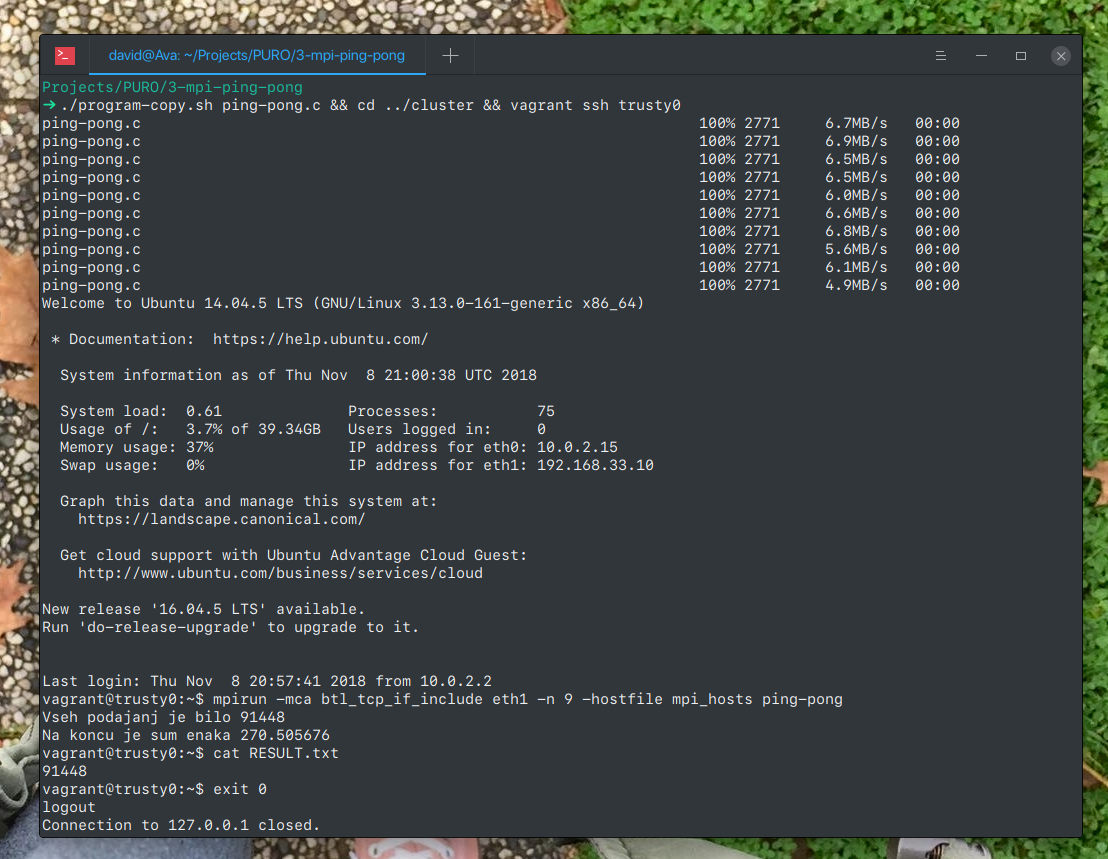
\includegraphics[scale=0.5]{./proof.png}
\caption{Delovanje programa pri 9 instancah}
\label{slika1}
\end{center}
\end{figure}

\section{Izjava o izdelavi domače naloge}
Domačo nalogo in pripadajoče programe sem izdelal sam.

\end{document}
